\subsection{Verifica della documentazione}
	Per la verifica della documentazione si utilizza la tecnica del \glock{walkthrough} revisionando i documenti per intero e la tecnica di \glock{inspection}.

\subsubsection{Calcolo leggibilità e controllo ortografia dei documenti}
	Per verificare quanto sono leggibili i documenti redatti si utilizza l'\glock{indice di Gulpease} ed è stato effettuato un controllo di ortografia. La seguente tabella contiene i risultati ottenuti all'ultima release dei documenti:

\begin{table} [h!]
	\rowcolors{2}{gray!25}{gray!6}
	\begin{center}
		\begin{tabular} { c c c c}
			\rowcolor{lightgray}
			\textbf{Documento}&\textbf{Errori ortografici}&\textbf{Indice di gulpease}&\textbf{Esito}\\
            \dext{Analisi dei requisiti v3.0.0}	& 0	& 71 &Superato\\
            \dext{Glossario v4.0.0}				& 0	& 48 &Superato\\
            \dext{Media verbali v1.0.0}			& 0	& 62 &Superato\\
            \dext{Norme di progetto v4.0.0} 	& 0	& 63 &Superato\\
            \dext{Piano di progetto v4.0.0}		& 0 & 53 &Superato\\
            \dext{Piano di qualifica v4.0.0}	& 0	& 45 &Superato\\
            \dext{Studio di fattibilità v1.0.0}	& 0	& 57 &Superato\\
		\end{tabular}
	\end{center}
	\caption{Esiti verifiche automatizzate - Revisione di Qualifica}
\end{table}

\subsection{MD01 - \glock{Indice di Gulpease}}

\begin{figure}[H]
	\centering
	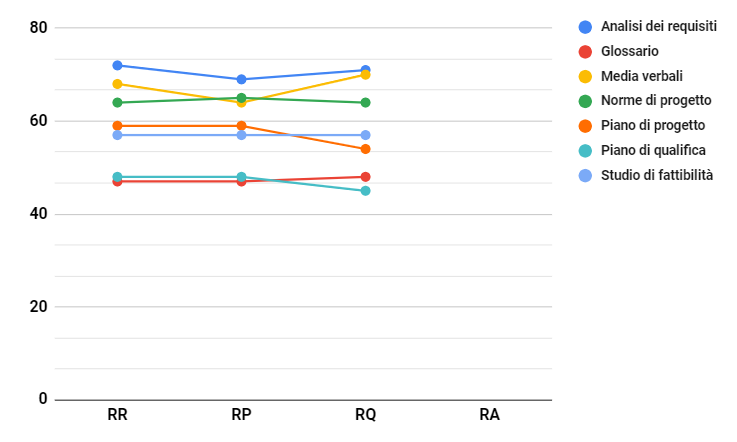
\includegraphics[width=12cm]{images/gulpease.png}
	\caption{Indice di gulpease per revisione}
\end{figure}

\subsection{MD02 - Correttezza ortografica}
\begin{figure}[H]
	\centering
	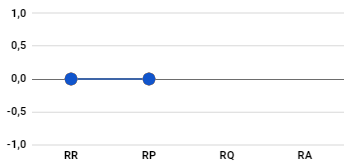
\includegraphics[width=9cm]{images/err_ortografici.png}
	\caption{Errori ortografici per revisione}
\end{figure}
\newpage

\subsection{Qualità di processo}

\subsubsection{MP01 - Schedule Variance}

\begin{figure}[H]
	\centering
	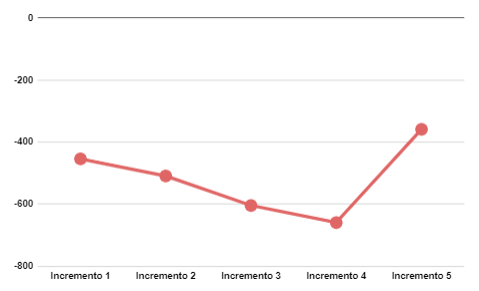
\includegraphics[width=11cm]{images/schedule_variance.png}
	\caption{Andamento metrica Schedule Variance}
\end{figure}

\subsubsection{MP02 - Cost Variance}

\begin{figure}[H]
	\centering
	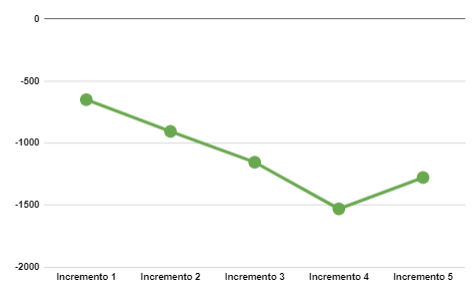
\includegraphics[width=11cm]{images/cost_variance.png}
	\caption{Andamento metrica Cost Variance}
\end{figure}

\subsubsection{MP03 - Budget Variance}

\begin{figure}[H]
	\centering
	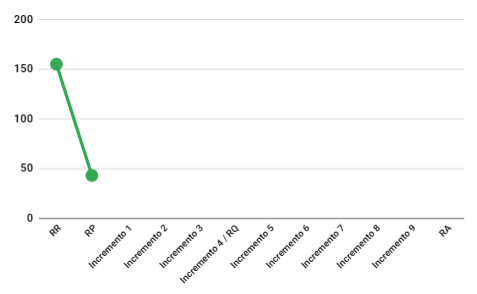
\includegraphics[width=11cm]{images/budget_variance.png}
	\caption{Andamento metrica Budget Variance}
\end{figure}



\subsubsection{MP04 - Unbudgeted Risks}

\begin{figure}[H]
	\centering
	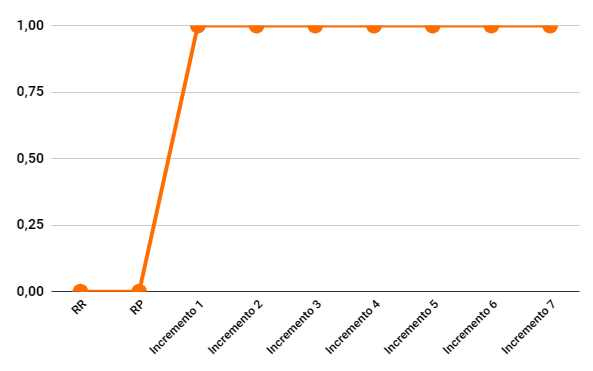
\includegraphics[width=11cm]{images/unbudgeted_risks.png}
	\caption{Andamento metrica Unbudgeted risks}
\end{figure}

\subsection{Qualità di prodotto}

\subsubsection{MS01 - Numero Bug Rilevati}
\begin{figure}[H]
	\centering
	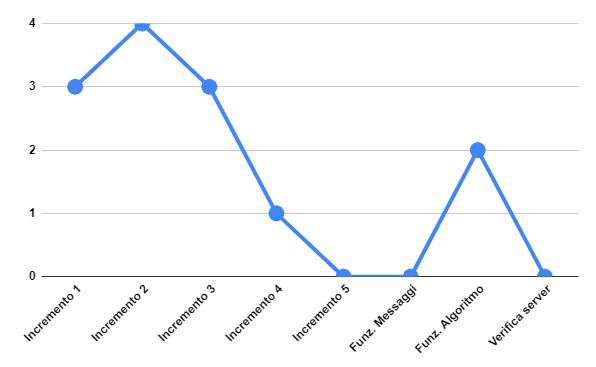
\includegraphics[width=10cm]{images/metricheServer/bug_rilevati.png}
	\caption{Andamento metrica Numero Bug Rilevati componente server}
\end{figure}
\begin{figure}[H]
	\centering
	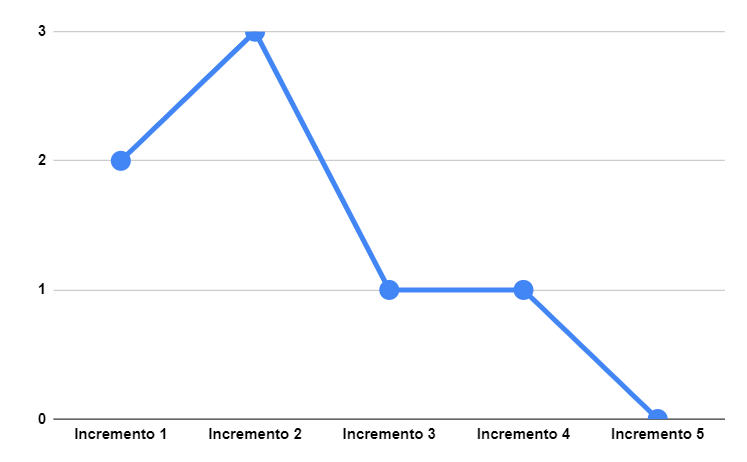
\includegraphics[width=10cm]{images/metricheUI/bug_rilevati.png}
	\caption{Andamento metrica Numero Bug Rilevati componente UI}
\end{figure}

\subsubsection{MS02 - Vulnerabilità}
\begin{figure}[H]
	\centering
	\includegraphics[width=10cm]{images/metricheServer/vulnerabilità.png}
	\caption{Andamento metrica Vulnerabilità componente server}
\end{figure}
\begin{figure}[H]
	\centering
	\includegraphics[width=10cm]{images/metricheUI/vulnerabilità.png}
	\caption{Andamento metrica Vulnerabilità componente UI}
\end{figure}

\subsubsection{MS03 - Code Smells}
\begin{figure}[H]
	\centering
	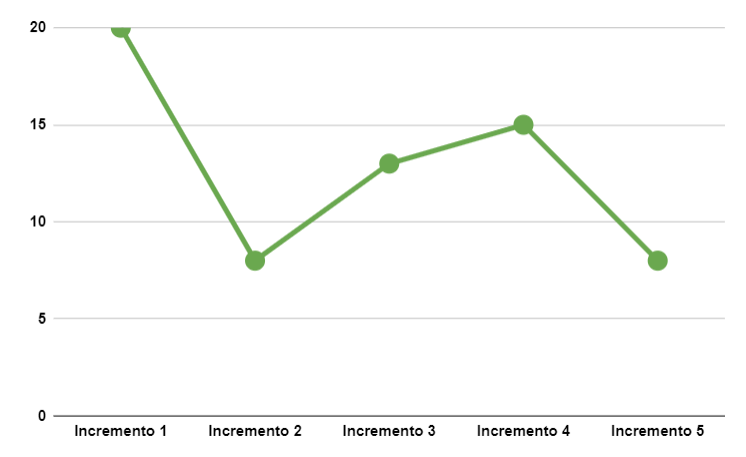
\includegraphics[width=10cm]{images/metricheServer/code_smells.png}
	\caption{Andamento metrica Code Smells componente server}
\end{figure}
\begin{figure}[H]
	\centering
	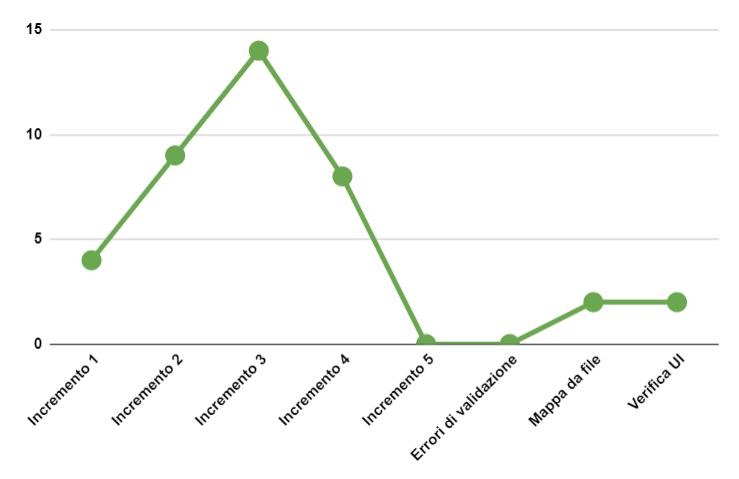
\includegraphics[width=10cm]{images/metricheUI/code_smells.png}
	\caption{Andamento metrica Code Smells componente UI}
\end{figure}
\newpage
\subsubsection{MS04 - Debito Tecnico}
\begin{figure}[H]
	\centering
	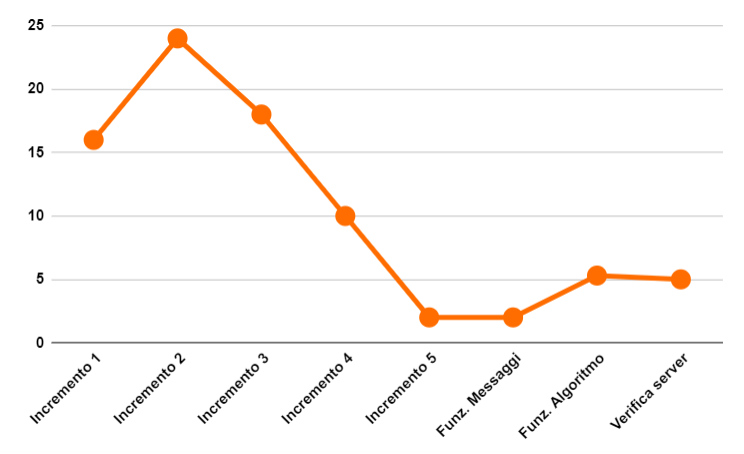
\includegraphics[width=10cm]{images/metricheServer/debito_tecnico.png}
	\caption{Andamento metrica Debito Tecnico componente server}
\end{figure}
\begin{figure}[H]
	\centering
	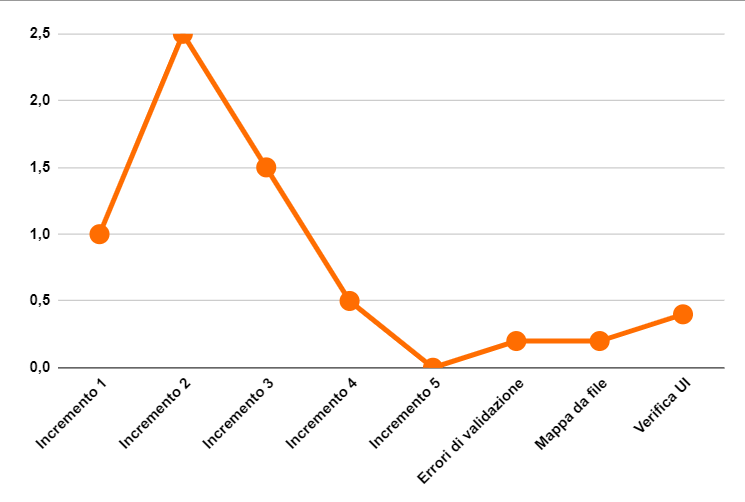
\includegraphics[width=10cm]{images/metricheUI/debito_tecnico.png}
	\caption{Andamento metrica Debito Tecnico componente UI}
	
\end{figure}

\subsubsection{MS05 - Complessità Ciclomatica}

\begin{figure}[H]
	\centering
	\includegraphics[width=10cm]{images/metricheServer/complessità_ciclomatica.png}
	\caption{Andamento metrica Debito Tecnico componente server}
\end{figure}
\begin{figure}[H]
	\centering
	\includegraphics[width=10cm]{images/metricheUI/complessità_ciclomatica.png}
	\caption{Andamento metrica Debito Tecnico componente UI}
\end{figure}

\subsubsection{MS06/MS07/MS08 - Requisiti Soddisfatti}
\begin{figure}[H]
	\centering
	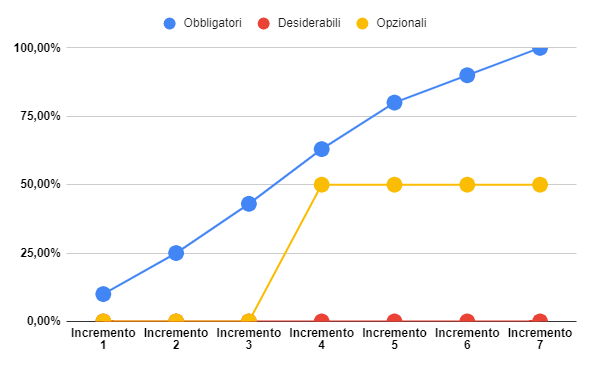
\includegraphics[width=11cm]{images/requisiti_soddisfatti.png}
	\caption{Andamento metrica Requisiti Soddisfatti}
\end{figure}

\subsubsection{MT01 - Code Coverage}

\begin{figure}[H]
	\centering
	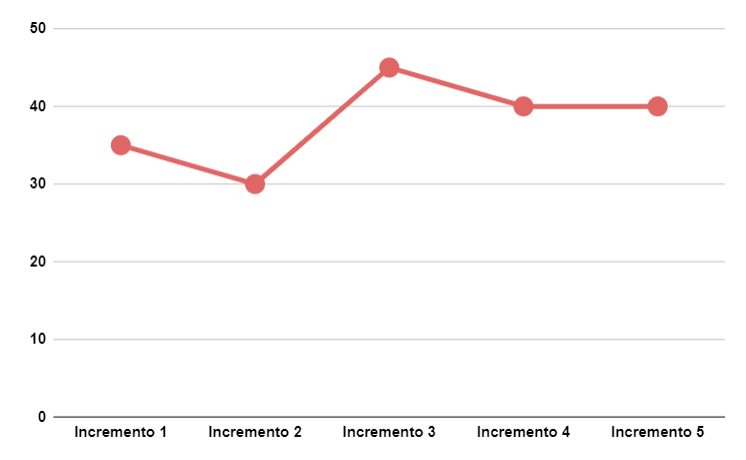
\includegraphics[width=10cm]{images/metricheServer/code_coverage.png}
	\caption{Andamento metrica Code Coverage componente server}
\end{figure}


\subsection{MT02 - Test di sistema implementati e superati}
\begin{figure}[H]
	\centering
	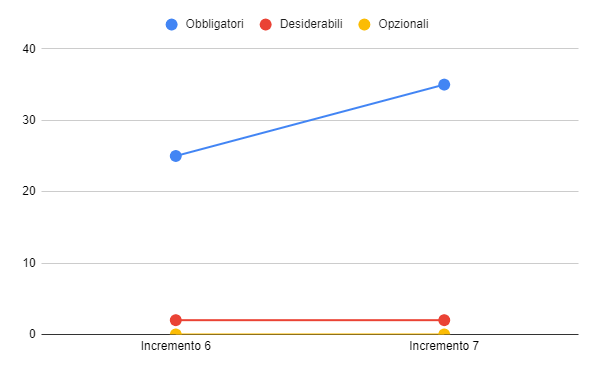
\includegraphics[width=11cm]{images/test/test_sistema.png}
	\caption{Test di sistema implementati e superati}
\end{figure}


\subsection{MT03 - Test di integrazione implementati e superati}
\begin{figure}[H]
	\centering
	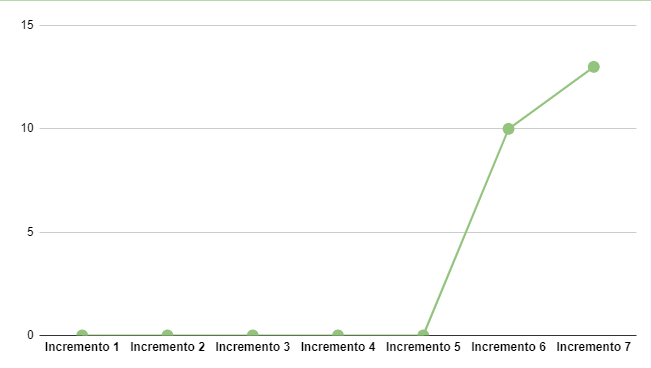
\includegraphics[width=11cm]{images/test/test_integrazione.png}
	\caption{Test di integrazione implementati e superati}
\end{figure}

\subsection{MT04 - Test di unità implementati e superati}
\begin{figure}[H]
	\centering
	\includegraphics[width=11cm]{images/test/test_unità.png}
	\caption{Test di unità implementati e superati}
\end{figure}